In this report, we describe the program we created to simulate a system of conveyor belts that transport luggage items.

The system could potentially be used as a tool for modelling for example a luggage system at an airport. However, we have decided to make our application more like a game, since a real simulation system would be difficult to make and furthermore require specialised domain knowledge about the system to simulate. This means that we provide conveyor belts that have a given friction with the luggage and all luggage items have the same size, weight and shape. In a proper simulation program, this should probably be somehow configurable by the user, but we consider that outside the scope of this project. The main focus in our program lies on user interaction and good visualisation. Hence, the program should be easy to use, it should not be hard to get to know the program and it should look good.

Before we started working on the project, we created a mock-up, as shown in Figure~\ref{fig:mockup}. Note that the arrows on the conveyor belts are purely there to indicate the direction in this sketchy figure, we intended to not show arrows from the start. Instead, we animate the conveyor belts and make it apparent to the user in that way in which direction a conveyor belt runs. Only when the user is placing new conveyor belts, in the so-called \emph{building mode}, we indicate with an arrow in which direction the user is building. The building mode (and the other modes in which the program can be) are described in more detail in Section~\ref{subsubsec:switch-program-modes}. The mock-up was part of a process in which we determined how the program should behave and what it should be able to do. The requirements that we set are described in the following section.

\begin{figure}[b!]
  \begin{center}
    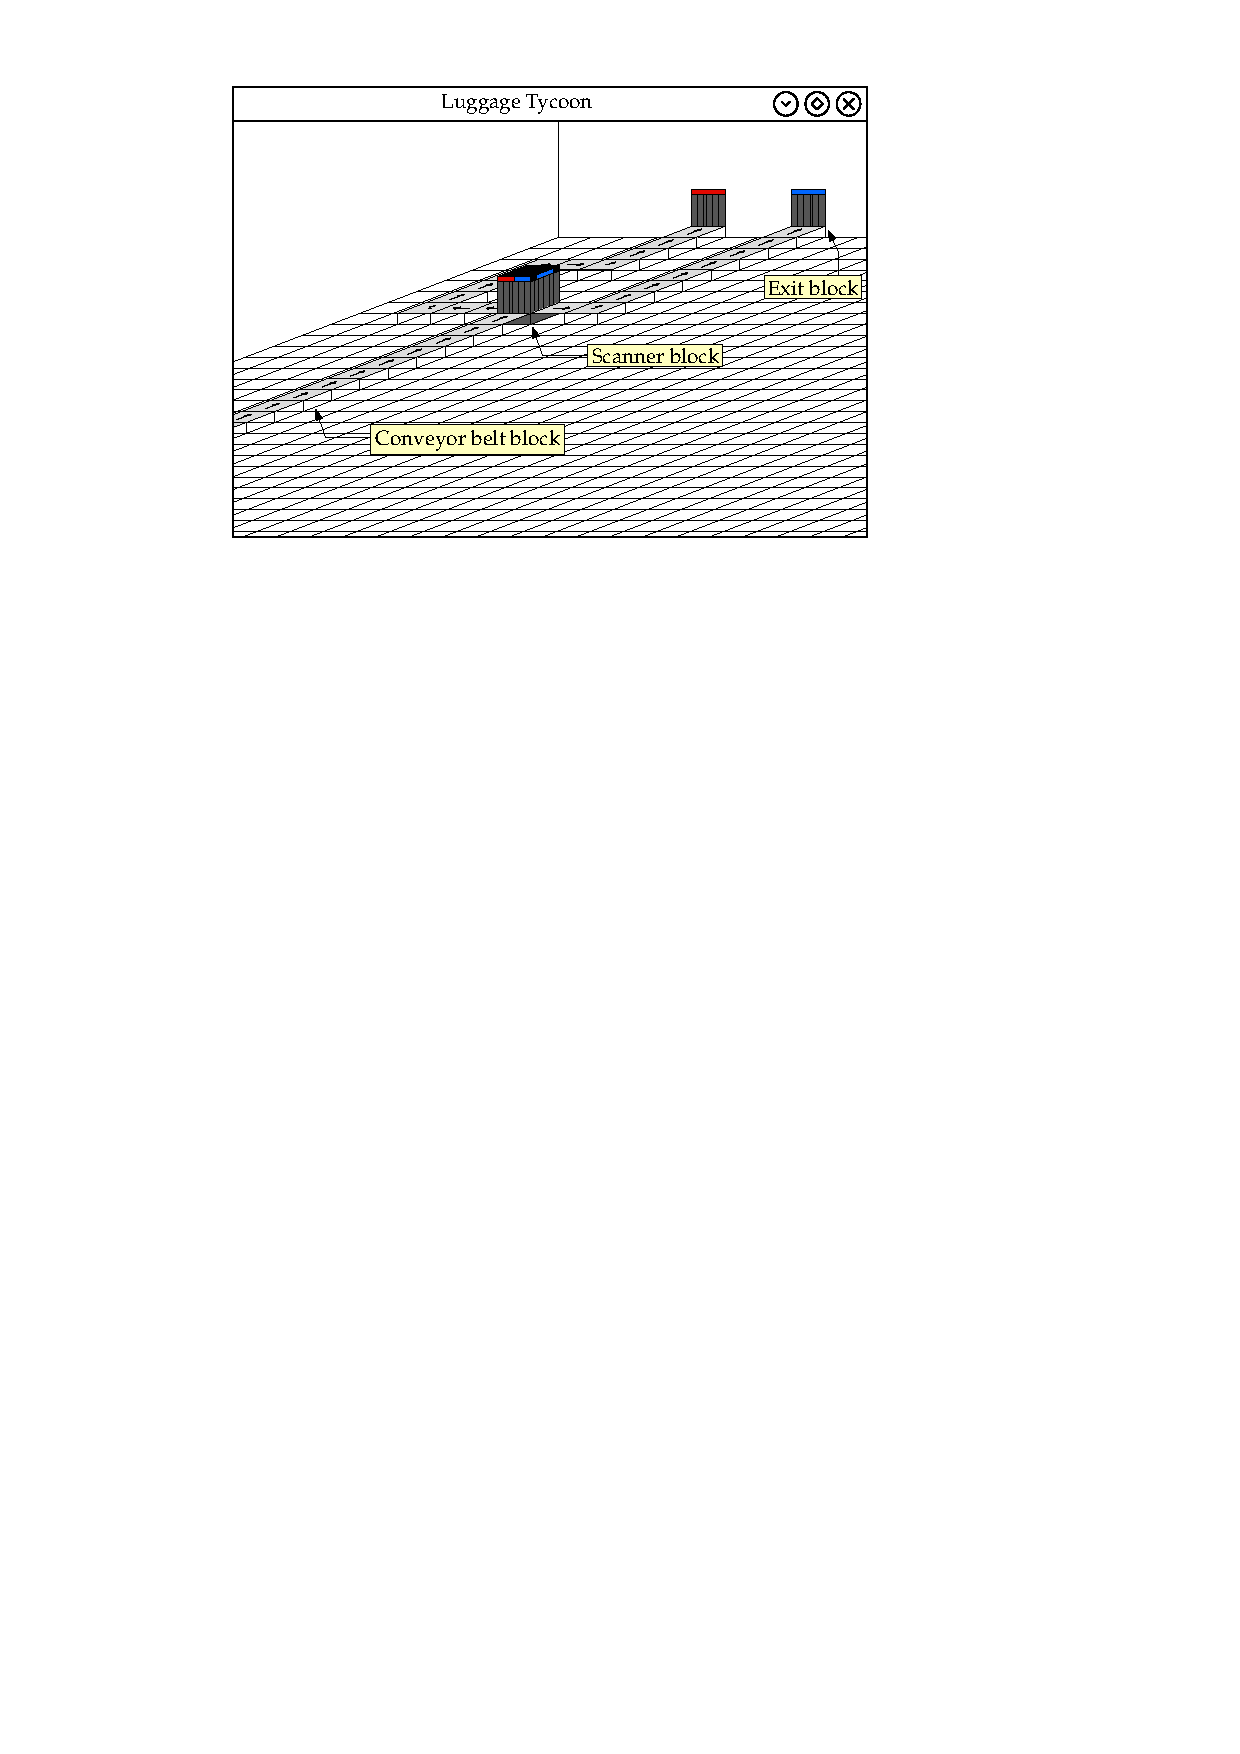
\includegraphics{mockup}
    \caption{A mock-up of the program we wanted to create.}
    \label{fig:mockup}
  \end{center}
\end{figure}

\subsection{Requirements}
The program that we built is a combination of an editor and a simulator: the user is able to construct a conveyor belt system in the editor, after which the movement of luggage in that system can be simulated.

\subsubsection{Design goals}
\textit{We will describe in this subsection what our goals are. Think of intuitive user interface, cross-platform, intended audience and possible use cases, \ldots}

First of all, we want the application to have a very intuitive interface, so that new users can easily find the functionality. Furthermore, we want the interface to be efficient, which means that frequent tasks (for example, building a long, straight conveyor belt) can be executed quickly by the user.

\subsubsection{Interaction}
\textit{In this subsection we present the way we implemented the aforementioned design goals or how we facilitate the mentioned intended audience and use cases. We may do so by including some small screenshots already or referring to Section~\ref{sec:results}.}
